\subsection{PAH intensities}
\label{sect:pah_ratios}

Both the 6.2 and 7.7~$\mu$m features are thought to be coming from ionized PAHs and the 11.3~$\mu$m feature from neutral PAHs. Therefore we expect to see a correlation between the intensities of 6.2 and 7.7~$\mu$m PAH features normalized by the 11.3~$\mu$m feature.  Figure \ref{PAHlines}  compares the PAH flux ratios of 7.7/11.3  and 6.2/11.3 features. The figure shows a good correlation between these two PAH line ratios, consistent with that of the SINGS sample shown by \citet{Smith:2007lr}.
A similar correlation was also reported by  \citet{Galliano2008} for a sample of galaxies and a handful of extended H{\sc ii} regions
and by \citet{Vermeij2002} for Galactic and Magellanic Cloud {\sc ii}regions. This provides evidence that the PAH emission from M31 is not unusual. 


\begin{figure}
\centering
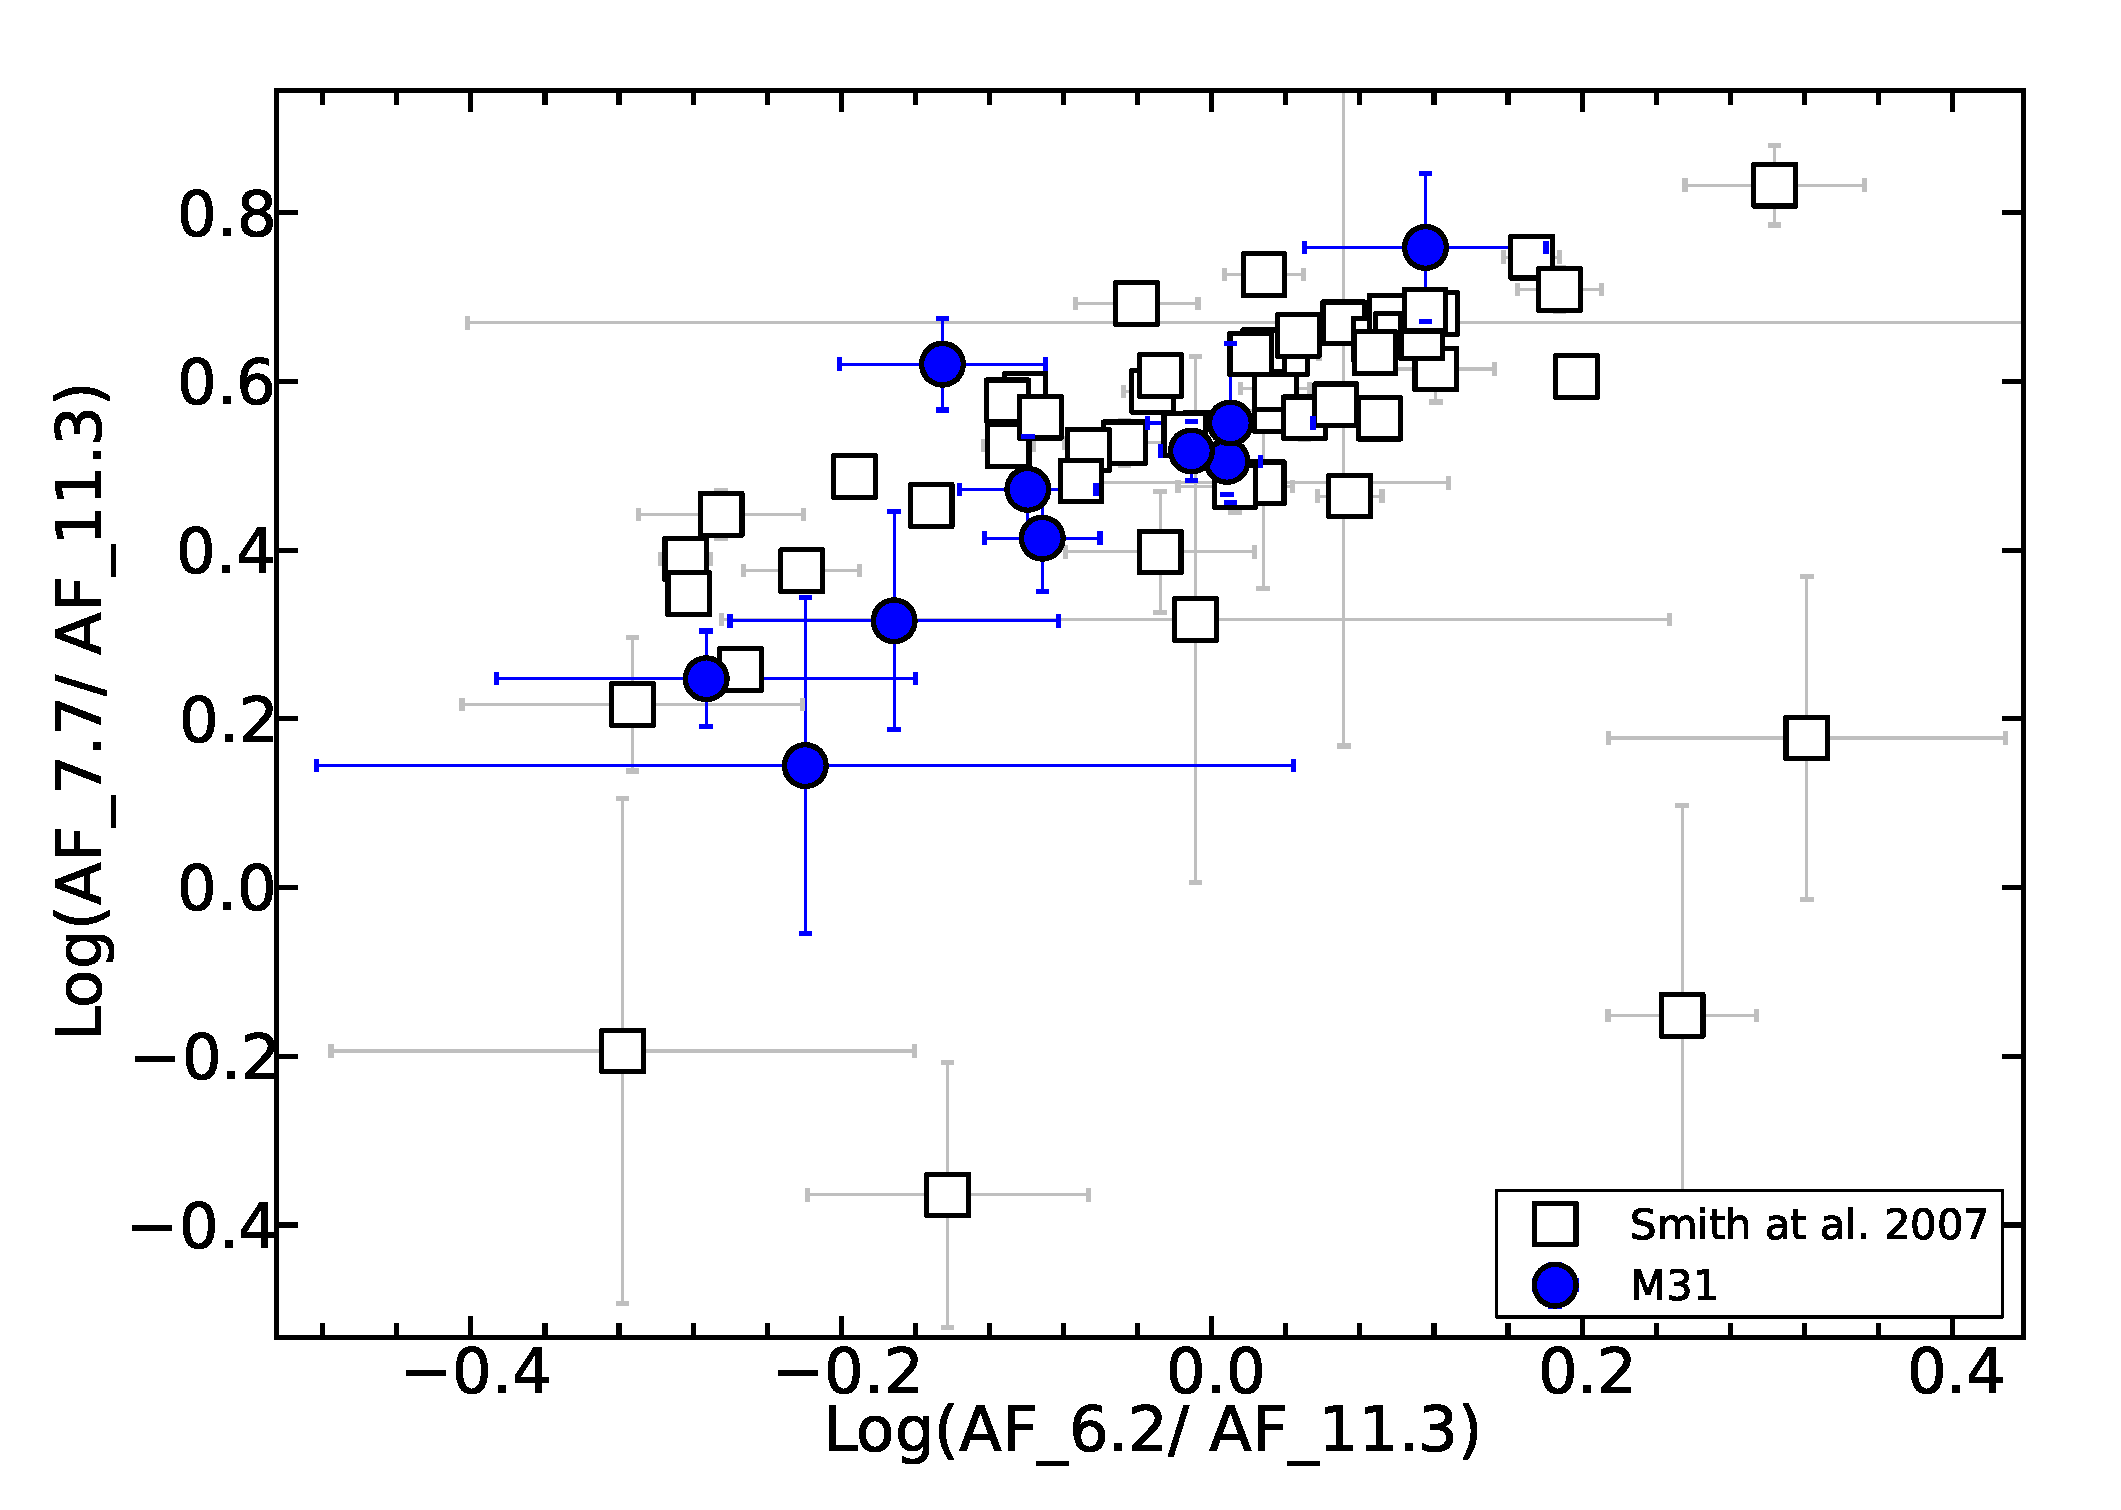
\includegraphics[scale = 0.25]{./SINGSnMy.eps}
\caption{Ratios of PAH feature fluxes (7.7~$\mu$m/11.3~$\mu$m versus 6.2~$\mu$m/11.3~$\mu$m) for 10 regions in M31.
Open squares represent the central regions of nearby galaxies as observed in the SINGS sample by \citet{Smith:2007lr}.
}
\label{PAHlines}
\end{figure}

\subsection{PAH equivalent widths versus radiation hardness}
\label{sect:eqw_rh}


\begin{figure}
\centering
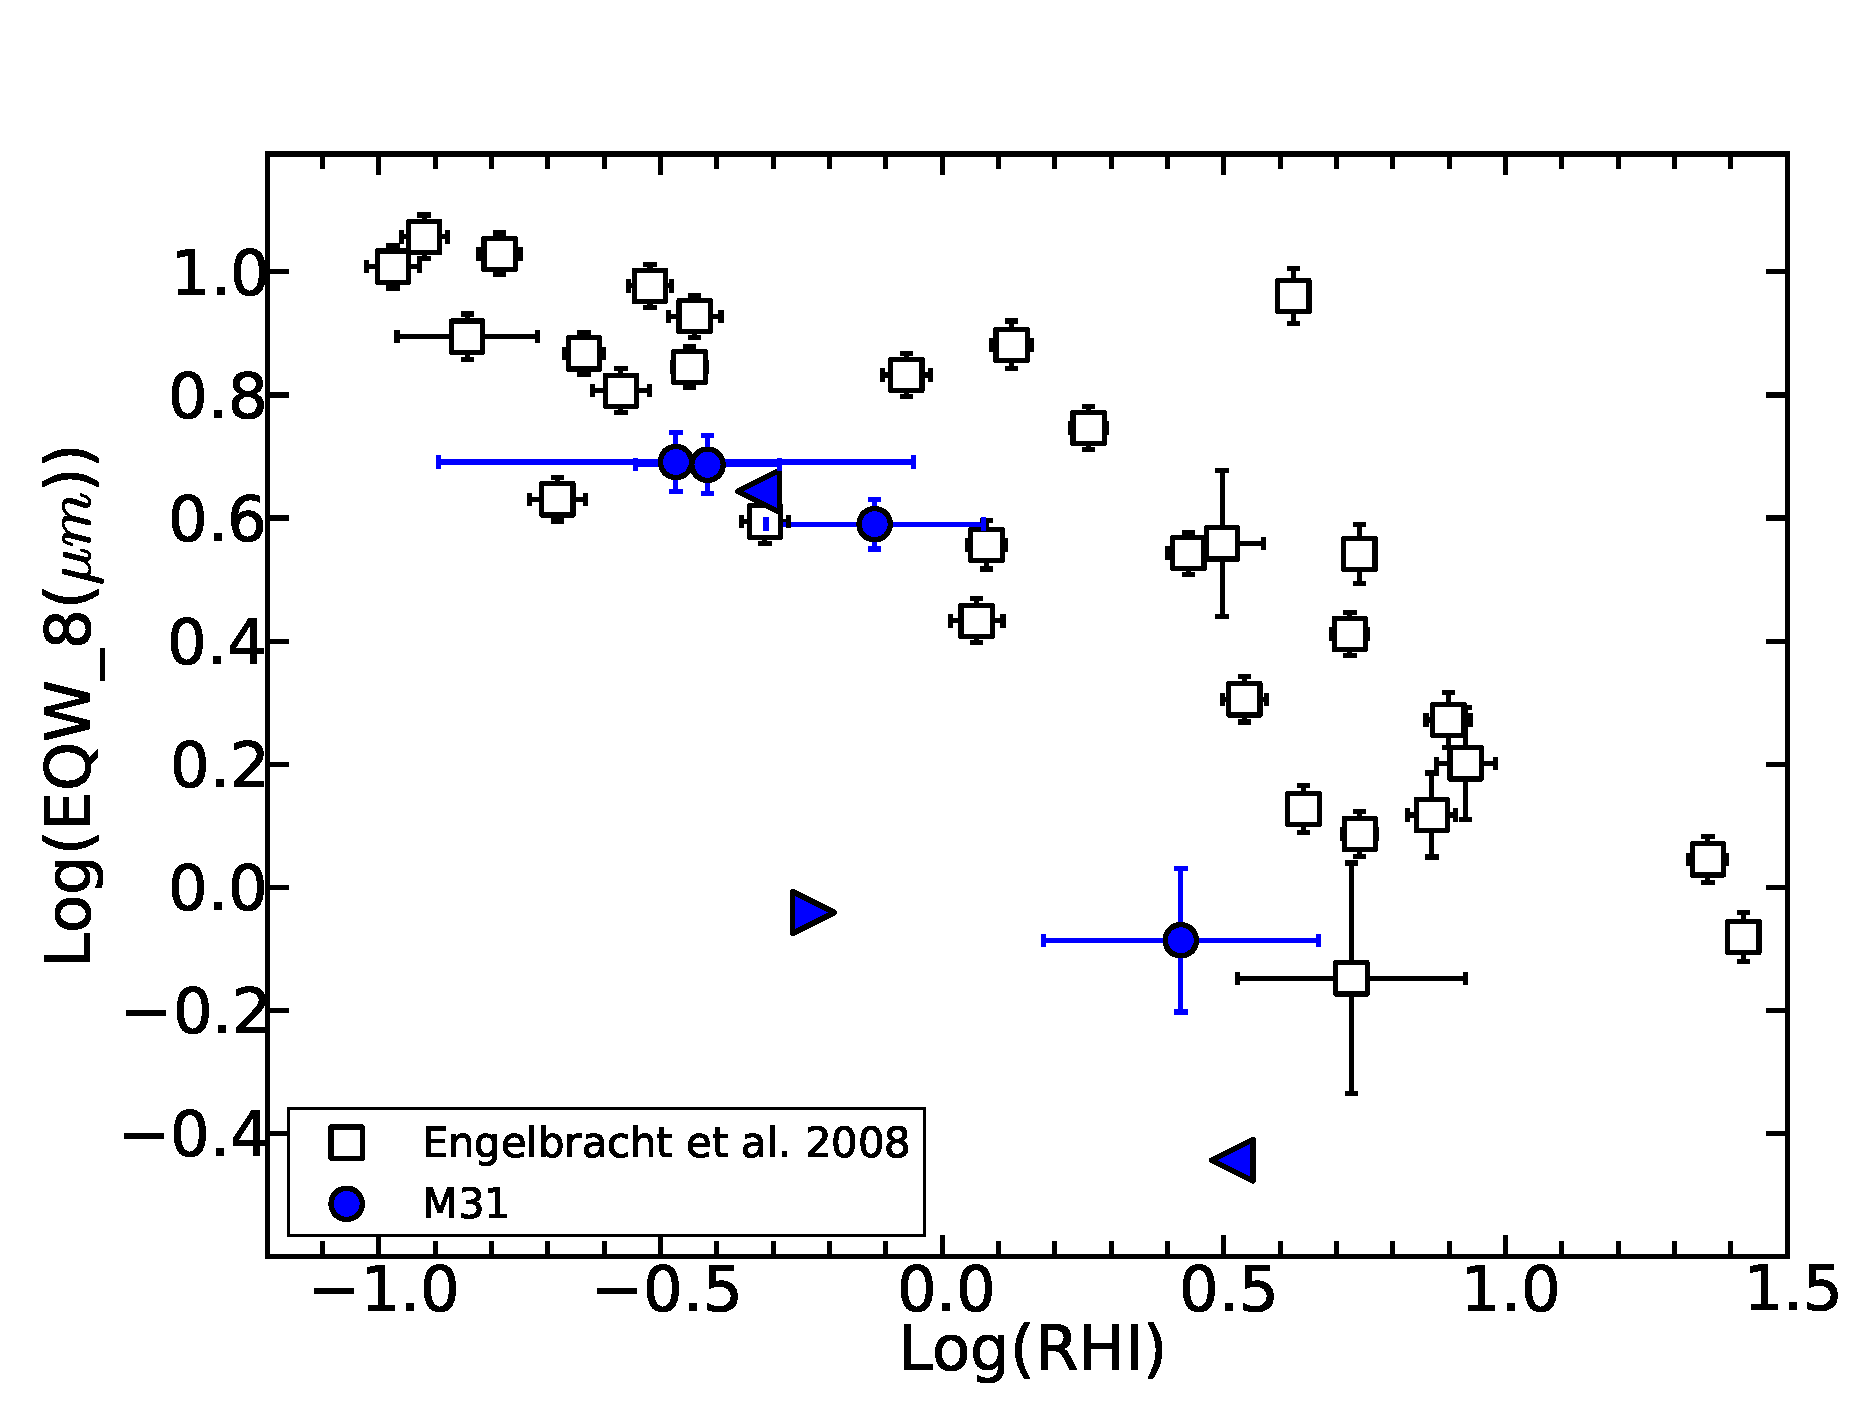
\includegraphics[scale=0.25]{./englvsmy.eps}
\caption{Equivalent width of the 8~$\mu$m PAH feature versus radiation hardness index (RHI) for the M31 sample (blue). 
The 8~$\mu$m feature is a combination of the 7.7, 8.3 and 8.6~$\mu$m PAHFIT components. 
Open squares represent the starburst galaxy sample from \citet{Engelbracht_2008}, which includes 66 nearby ($2<d<250$~Mpc)
star-bursting or star-forming galaxies selected to cover a wide range in metallicity ($7.1<12+\log{\rm[O/H]}<8.9$).
 For M31 spectra with undetected lines, triangles represent $3\sigma$ upper (left-pointing triangles) and lower (right-pointing triangles)  limits.} 
\label{englII}
\end{figure}

\begin{figure}
\centering
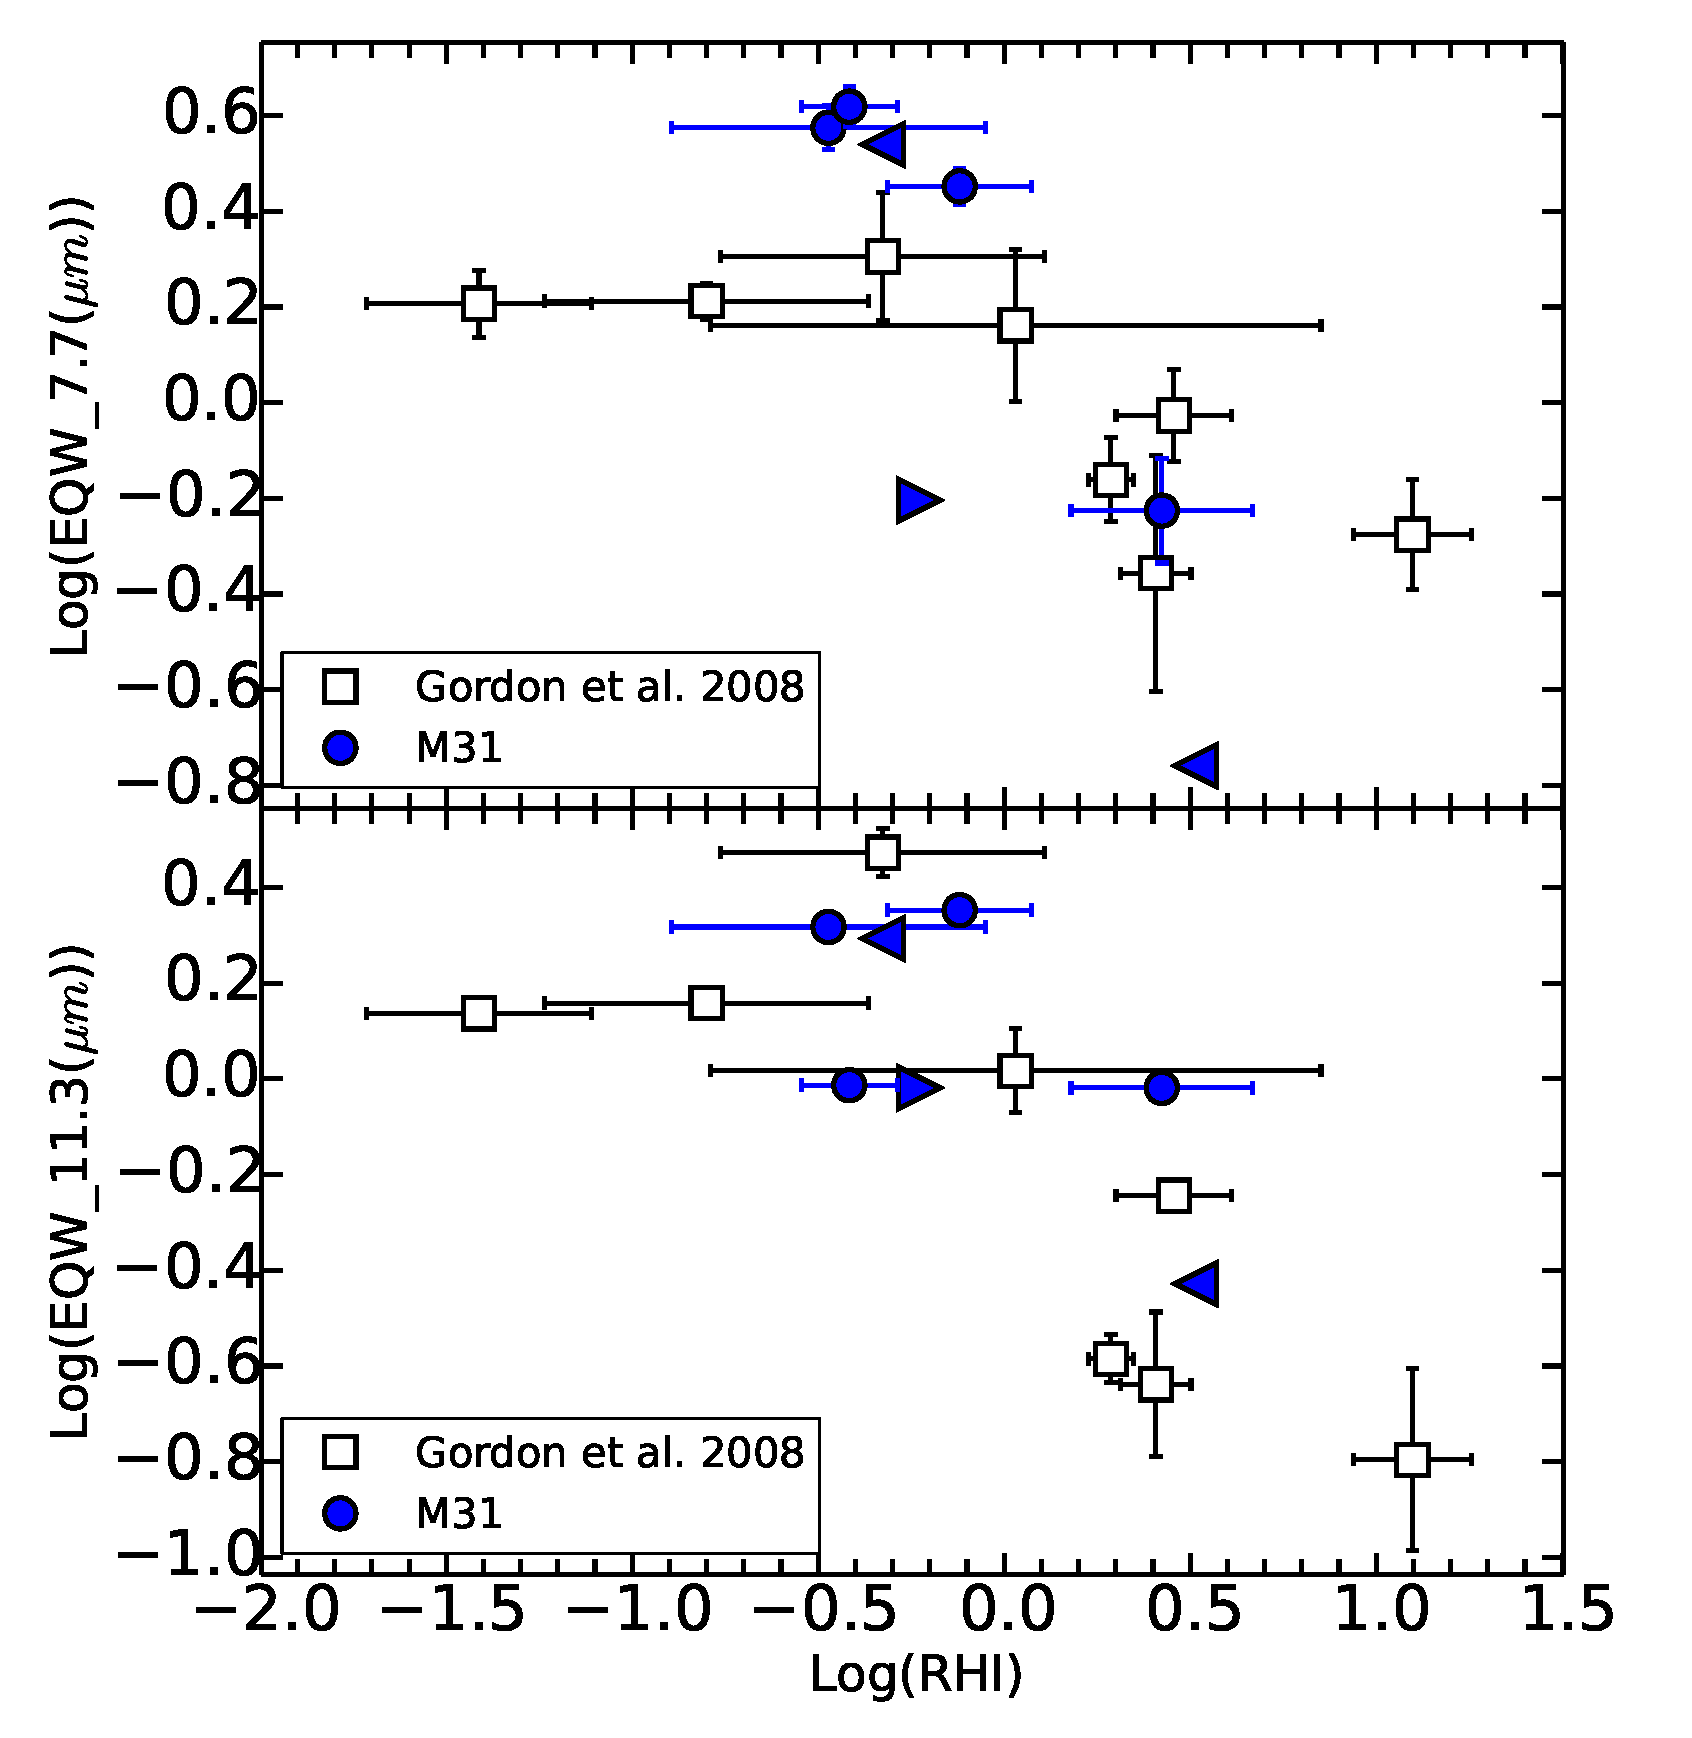
\includegraphics[scale=0.30]{./Gordvsmy.eps}
\caption{Equivalent widths of the normalized 7.7~$\mu$m PAH feature (top panel) and 11.3~$\mu$m PAH feature (bottom panel) versus 
radiation hardness index (RHI) for the M31 sample. Open squares represent the seven H~{\sc ii} regions in M101 observed  by \citet{Gordon:2008lr},  
which have $8.1<12+\log{\rm[O/H]}<8.8$ 
The normalization was done by dividing each EQW by the weighted average over all regions in the respective samples. 
Triangles represent $3\sigma$ upper and lower limits.} 
\label{gordII}
\end{figure}


As mentioned in the introduction, PAH equivalent widths tend to show an inverse correlation with radiation hardness. 
The equivalent widths of the M31 PAH features are compared with RHI in Figures~\ref{englII} and \ref{gordII}.
For reference, we also show the starburst sample of \citet{Engelbracht_2008} 
and the seven H~{\sc ii} regions in M101 observed by \citet{Gordon:2008lr}.
To make a direct comparison with the M101 sample, we normalized the M31 EQWs in Figure~\ref{gordII} using the same procedure
as \citet{Gordon:2008lr}, dividing each EQW by the  weighted average over all regions in the respective samples. 
The equivalent widths seem to be decreasing with increasing radiation hardness, consistent with previous results. 
This also helps to confirm that the PAH emission in M31 is not unusual. 


\subsection{PAH equivalent widths versus metallicity}
\label{sect:eqw_met}

Many studies based on ISO and {\em Spitzer} observations have reported that PAH intensity decreases with decreasing metallicity \citep{Calzetti:2010fk}. 
In addition, these studies also report a sudden drop of EQWs of PAHs around $12+\log{\rm (O/H)} \approx 8.1$. 
This has been observed amongst different galaxies \citep{Engelbracht_2008} as well as within a single galaxy \citep{Gordon:2008lr}. 

\citet{Sanders_2011}  measured spectroscopic metallicities for
more than 250 H~{\sc ii} regions using strong line diagnostics.\footnote{\citet{Sanders_2011} considered several different
calibrations for abundance diagnostics. We use the results from the method they denote ``N06 N2''  \citep{Nagao2006} because
that method has the largest sample size.} Except for regions 5 and 8, all of our mapped regions contain an  H~{\sc ii} region measured by
 \citet{Sanders_2011}, and we give the corresponding metallicities in Table~\ref{regions}.
 For regions 5 and 8 we adopted metallicities from the radial metallicity profile of M31 given by
 \citet{Sanders_2011}. It is well known that there are systematic differences between different 
 methods used to measure metallicities, and those in the sample of \citet{Engelbracht_2008} 
 were obtained by the direct electron temperature method  \citep{Skillman1998}.
\citet{Mitchel2014} calculated the offset between direct and strong-line measurements for M31 H~{\sc ii} regions to be 
$0.35\pm0.10$ and we correct for this in Figure~\ref{metalicityVseqw}.

\begin{figure}
\centering
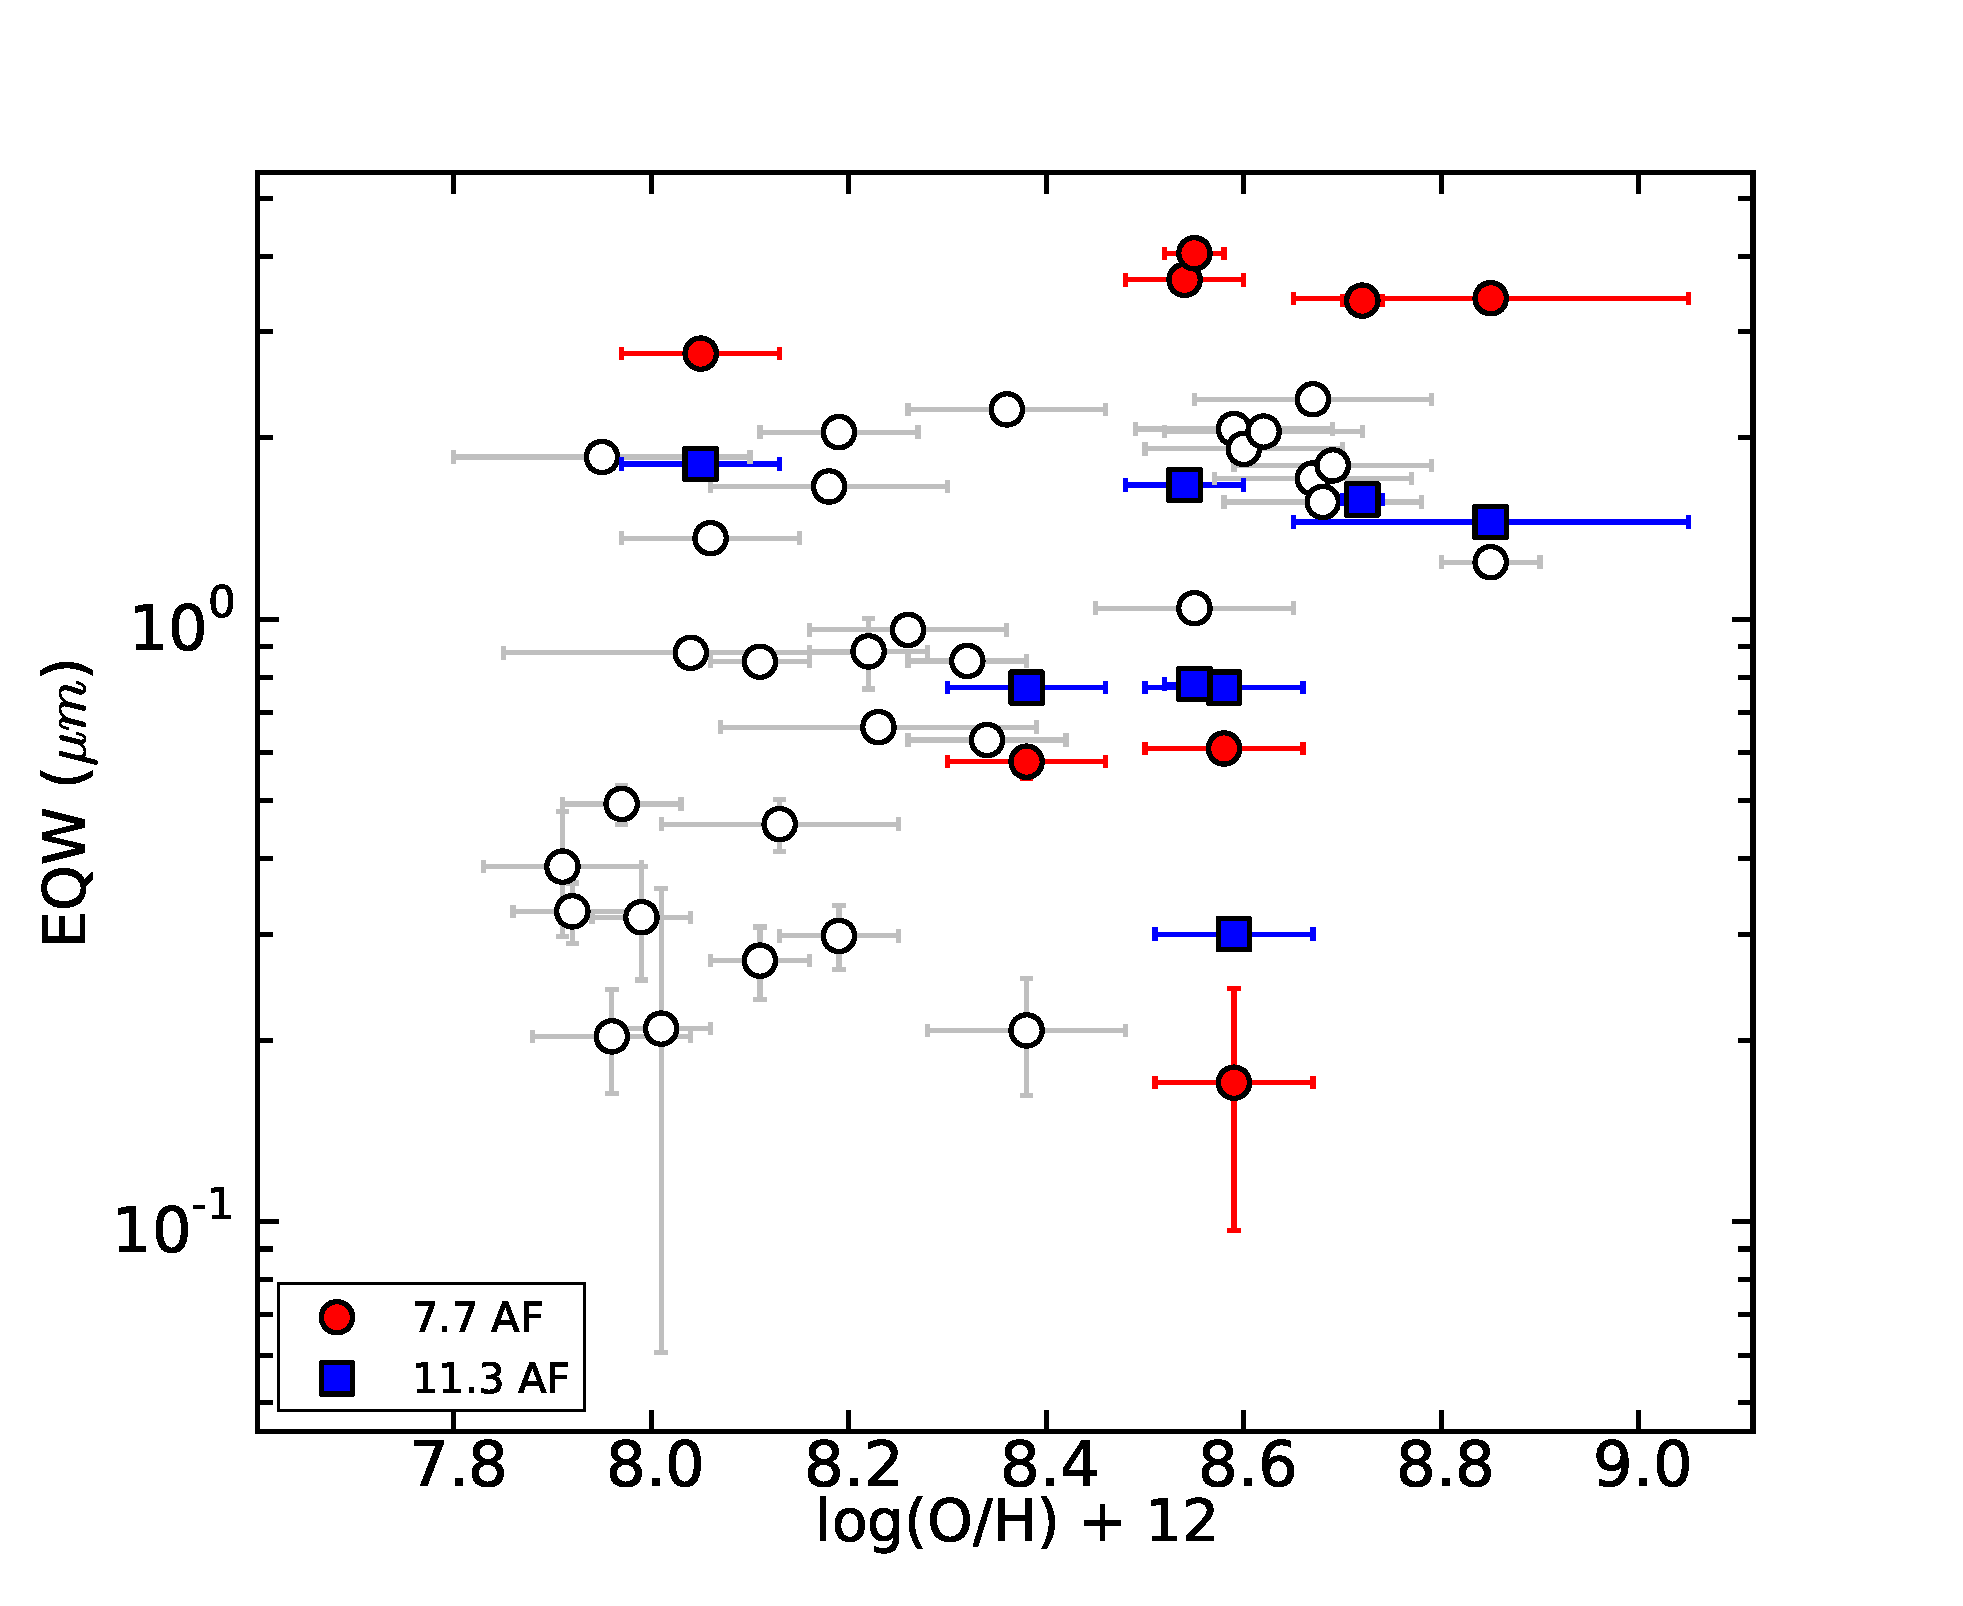
\includegraphics[scale=0.27]{./oxyvseqw.eps}
\caption{ PAH equivalent widths versus metallicity. 
Filled circles are M31 7.7~$\mu$m EQWs; filled squares are M31 11.3~$\mu$m EQWs; 
open circles are 7.7~$\mu$m EQWs for the starburst sample from \citet{Engelbracht_2008}.
Metallicities of the M31 regions have had 0.35~dex subtracted to account for the offset  between direct and strong-line measurements. 
}
\label{metalicityVseqw}
\end{figure}

Figure \ref{metalicityVseqw} shows the normalized EQWs of the PAH features  versus the metallicity for our sample and the starburst 
galaxies of \citet{Engelbracht_2008}. The scatter in our sample is large, but the 	
equivalent widths of the 7.7 and 11.3~$\mu$m features are consistent with those of \citet{Engelbracht_2008}. 
No trend with metallicity is seen.
However, we do not have enough data from low-metallicity regions in M31 to observe the expected decrease of EQWs of PAH with the decreasing 
metallicity.  There do seem to be some outliers which can plausibly be due to the uncertainties  and the offset between different methods of calculating the metallicity.  
The M31 region with very low  7.7~$\mu$m  equivalent widths is Region 8, which has
a noisy spectrum in the blue as well as substantial modelled contribution from starlight (see Figure~\ref{PAHFITplots}).

